\newacronym{iae}{IAE}{\textit{Integral Absolute Error}}
\newacronym{ise}{ISE}{\textit{Integral Square Error}}
\newacronym{itae}{ITAE}{\textit{Integral Time Absolute Error}}
\newacronym{itse}{ITSE}{\textit{Integral Time Square Error}}

\chapter{Resultados}
\label{ch:resultados}

Para a aplicação dos controladores \acrshort{mpc} criados nos capítulos anteriores, foi desenvolvido um
ambiente \textit{Simulink} (\cref{fig:simulinkusingmpc}) onde cada um dos diferentes controladores obtidos
foram conectados ao \acrshort{tclabsp} para realizar seu controle.

Todos\footnote{
    O \acrshort{matlab} não conseguiu criar um controlador baseado no modelo experimental Box-Jenkins
    pois este modelo possui pólos discretizados próximos de $z=0$.
}  os diferentes controladores foram submetidos aos mesmos sinais de referência (\textit{set-point})
e ao mesmo tempo de experimento. Os sinais de referência utilizados foram sinais de amplitude randômica
e com duração de duas vezes o tempo de acomodação da planta em malha aberta, ou seja, $2$ x $T_s = 2$ x $383s = 766s$.
A duração do experimento foi determinada de forma que cinco sinais de entrada distintos pudessem ser
aplicados ao sistema, sendo assim o tempo dos experimentos foi de $5$ x $766s = 3830s$.
Cada um dos experimentos foi repetido ao menos 3 vezes e ao final foi calculada uma média de todos os 
sinais coletados para atenuar possíveis erros pontuais de cada experimento.

\begin{figure}[!h]
	\caption{Ambiente Simulink para implementação dos controladores MPC}
	\begin{center}
		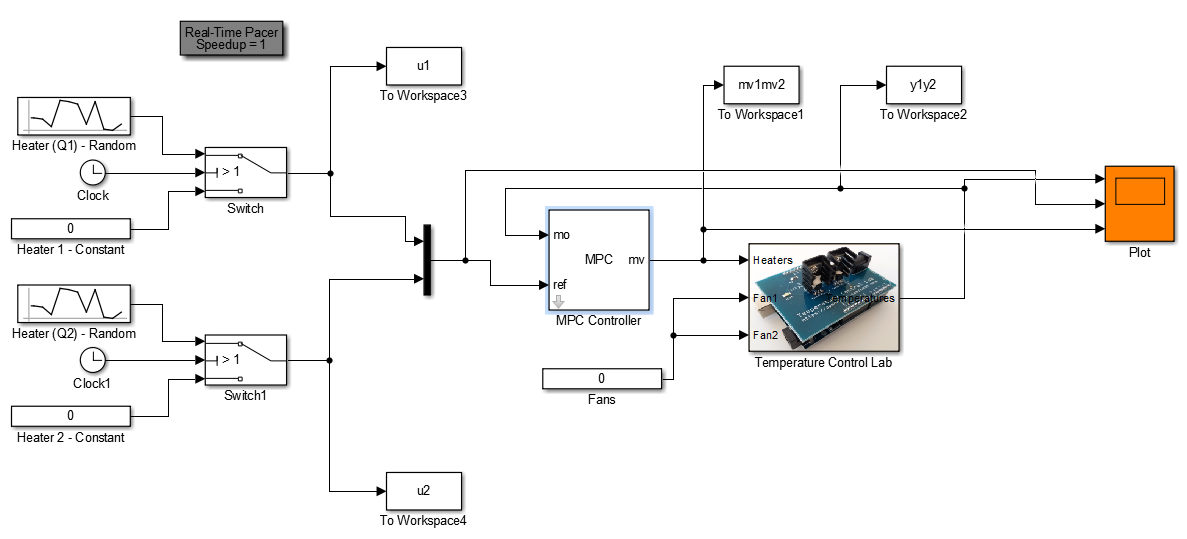
\includegraphics[width=1.00\textwidth]{./5_images/SimulinkUsingMPC.png} 
		\label{fig:simulinkusingmpc}
	\end{center}
	\centering
	\makebox[\width]{Fonte: Autor} 
\end{figure}

As \crefrange{fig:resultadosmpc-teoss}{fig:resultadosmpc-exparx} apresentam os gráficos de resposta em malha fechada
para cada um dos experimentos aplicando os modelos obtidos. Para fins comparativos, a \cref{fig:resultadospid}
apresenta o gráfico de resposta do controlador \acrshort{pid} apresentado na \cref{sec:controlador_pid}.

\begin{figure}[!h]
	\caption{Resposta do controlador MPC criado a partir do modelo teórico}
	\begin{center}
		\includegraphics[width=1.00\textwidth]{./5_images/ResultadosMPC-TeoSS.eps} 
		\label{fig:resultadosmpc-teoss}
	\end{center}
	\centering
	\makebox[\width]{Fonte: Autor} 
\end{figure}

\begin{figure}[!h]
	\caption{Resposta do controlador MPC criado a partir do modelo experimental (função de transferência)}
	\begin{center}
		\includegraphics[width=1.00\textwidth]{./5_images/ResultadosMPC-ExpTF.eps} 
		\label{fig:resultadosmpc-exptf}
	\end{center}
	\centering
	\makebox[\width]{Fonte: Autor} 
\end{figure}

\begin{figure}[!h]
	\caption{Resposta do controlador MPC criado a partir do modelo experimental (ARMAX)}
	\begin{center}
		\includegraphics[width=1.00\textwidth]{./5_images/ResultadosMPC-ExpARMAX.eps} 
		\label{fig:resultadosmpc-exparmax}
	\end{center}
	\centering
	\makebox[\width]{Fonte: Autor} 
\end{figure}

\begin{figure}[!h]
	\caption{Resposta do controlador MPC criado a partir do modelo experimental (Output-Error)}
	\begin{center}
		\includegraphics[width=1.00\textwidth]{./5_images/ResultadosMPC-ExpOE.eps} 
		\label{fig:resultadosmpc-expoe}
	\end{center}
	\centering
	\makebox[\width]{Fonte: Autor} 
\end{figure}

\begin{figure}[!h]
	\caption{Resposta do controlador MPC criado a partir do modelo experimental (espeço de estados)}
	\begin{center}
		\includegraphics[width=1.00\textwidth]{./5_images/ResultadosMPC-ExpSS.eps} 
		\label{fig:resultadosmpc-expss}
	\end{center}
	\centering
	\makebox[\width]{Fonte: Autor} 
\end{figure}

\begin{figure}[!h]
	\caption{Resposta do controlador MPC criado a partir do modelo experimental (ARX)}
	\begin{center}
		\includegraphics[width=1.00\textwidth]{./5_images/ResultadosMPC-ExpARX.eps} 
		\label{fig:resultadosmpc-exparx}
	\end{center}
	\centering
	\makebox[\width]{Fonte: Autor} 
\end{figure}

\clearpage

\begin{figure}[!h]
	\caption{Resposta do controlador PID auto-sintonizado}
	\begin{center}
		\includegraphics[width=1.00\textwidth]{./5_images/ResultadosPID.eps} 
		\label{fig:resultadospid}
	\end{center}
	\centering
	\makebox[\width]{Fonte: Autor} 
\end{figure}

Nas \crefrange{tab:resultados_mpc_e_pid_iae}{tab:resultados_mpc_e_pid_itse} é possível observar diferentes indicadores
de performance para cada um dos modelos testados.

Os indicadores utilizados são:

\begin{itemize}
	\item \acrshort{iae}: Integral absoluta do erro (do inglês \acrlong{iae})
		\begin{align}
			IAE = \int_{0}^{\infty} \mid e \mid dt			\label{eq:iae}
		\end{align}
	\item \acrshort{ise}: Integral quadrada do erro (do inglês \acrlong{ise})
		\begin{align}
			ISE = \int_{0}^{\infty} e^{2} dt				\label{eq:ise}
		\end{align}
	\item \acrshort{itae}: Integral absoluta do erro no tempo (do inglês \acrlong{itae})
		\begin{align}
			ITAE = \int_{0}^{\infty} t \mid e \mid dt		\label{eq:itae}
		\end{align}
	\item \acrshort{itse}: Integral quadrada do erro no tempo (do inglês \acrlong{itse})
		\begin{align}
			ITSE &= \int_{0}^{\infty} t \cdot e^{2} dt		\label{eq:itse}
		\end{align}
\end{itemize}

% \clearpage

\begin{table}[!h]
	\centering
	\caption{Performance dos controladores \acrshort{mpc} e \acrshort{pid} - IAE}
	\label{tab:resultados_mpc_e_pid_iae}
	\begin{tabular}{l|cc|c} \toprule
		{Modelo utilizado no controlador}              			            &	\begin{tabular}[c]{@{}c@{}}Sensor 1\\(x$10^3$)\end{tabular}		&	\begin{tabular}[c]{@{}c@{}}Sensor 2\\(x$10^3$)\end{tabular}     		& \begin{tabular}[c]{@{}c@{}}Média\\(x$10^3$)\end{tabular}		\\ \midrule
		MPC Teórico \acrshort{ss} (\cref{eq:tclab_modelo_teorico})	        &   $38.07$           												&   $27.94$          														&   $33.00$														\\ 
		MPC Experimental \acrshort{oe} (\cref{tab:tclabsp-model-oe})	    &   $45.53$           												&   $42.16$          														&   $43.85$														\\ 
		MPC Experimental \acrshort{armax} (\cref{tab:tclabsp-model-armax})	&   $58.16$           												&   $37.27$          														&   $47.72$														\\ 
		MPC Experimental \acrshort{tf} (\cref{tab:tclabsp-model-tf})		&   $56.90$           												&   $55.08$          														&   $55.99$														\\ 
		PID (\cref{tab:pid_values})	                                        &   $53.90$           												&   $59.10$          														&   $56.50$														\\ 
		MPC Experimental \acrshort{arx}	(\cref{tab:tclabsp-model-arx})		&   $59.13$           												&   $63.35$          														&   $61.24$														\\ 
		MPC Experimental \acrshort{ss} (\cref{eq:tclabsp-model-ss})			&   $75.99$           												&   $58.12$          														&   $67.06$														\\ \bottomrule 
	\end{tabular}
	\caption*{Fonte: Autor}
\end{table}   

\begin{table}[!h]
	\centering
	\caption{Performance dos controladores \acrshort{mpc} e \acrshort{pid} - ISE}
	\label{tab:resultados_mpc_e_pid_ise}
	\begin{tabular}{l|cc|c} \toprule
		{Modelo utilizado no controlador}              			            &	\begin{tabular}[c]{@{}c@{}}Sensor 1\\(x$10^4$)\end{tabular}		&	\begin{tabular}[c]{@{}c@{}}Sensor 2\\(x$10^4$)\end{tabular}     		& \begin{tabular}[c]{@{}c@{}}Média\\(x$10^4$)\end{tabular}			\\ \midrule
		MPC Teórico \acrshort{ss} (\cref{eq:tclab_modelo_teorico})	        &   $62.95$           												&   $29.03$          														&   $45.99$															\\ 
		MPC Experimental \acrshort{oe} (\cref{tab:tclabsp-model-oe})	    &   $66.46$           												&   $32.78$          														&   $49.62$															\\ 
		MPC Experimental \acrshort{armax} (\cref{tab:tclabsp-model-armax})	&   $77.46$           												&   $30.68$          														&   $54.07$															\\ 
		MPC Experimental \acrshort{tf} (\cref{tab:tclabsp-model-tf})		&   $76.61$           												&   $39.75$          														&   $58.18$															\\ 
		MPC Experimental \acrshort{arx}	(\cref{tab:tclabsp-model-arx})		&   $67.98$           												&   $49.01$          														&   $58.50$															\\ 
		MPC Experimental \acrshort{ss} (\cref{eq:tclabsp-model-ss})			&   $81.04$           												&   $40.95$          														&   $61.00$															\\ 
		PID (\cref{tab:pid_values})	                                        &   $76.83$           												&   $50.06$          														&   $63.45$															\\ \bottomrule 
	\end{tabular}
	\caption*{Fonte: Autor}
\end{table}

\begin{table}[!h]
	\centering
	\caption{Performance dos controladores \acrshort{mpc} e \acrshort{pid} - ITAE}
	\label{tab:resultados_mpc_e_pid_itae}
	\begin{tabular}{l|cc|c} \toprule
		{Modelo utilizado no controlador}              			            &	\begin{tabular}[c]{@{}c@{}}Sensor 1\\(x$10^6$)\end{tabular}		&	\begin{tabular}[c]{@{}c@{}}Sensor 2\\(x$10^6$)\end{tabular}     		& \begin{tabular}[c]{@{}c@{}}Média\\(x$10^6$)\end{tabular}			\\ \midrule
		MPC Teórico \acrshort{ss} (\cref{eq:tclab_modelo_teorico})	        &   $60.99$           												&   $38.11$          														&   $49.55$ 														\\ 
		MPC Experimental \acrshort{oe} (\cref{tab:tclabsp-model-oe})	    &   $73.78$           												&   $61.69$          														&   $67.74$ 														\\ 
		MPC Experimental \acrshort{armax} (\cref{tab:tclabsp-model-armax})	&   $91.79$           												&   $57.31$          														&   $74.55$ 														\\ 
		PID (\cref{tab:pid_values})	                                        &   $84.97$           												&   $88.90$          														&   $86.94$ 														\\ 
		MPC Experimental \acrshort{tf} (\cref{tab:tclabsp-model-tf})		&   $90.39$           												&   $84.58$          														&   $87.49$ 														\\ 
		MPC Experimental \acrshort{arx}	(\cref{tab:tclabsp-model-arx})		&   $105.79$           												&   $113.15$          														&   $109.47$														\\ 
		MPC Experimental \acrshort{ss} (\cref{eq:tclabsp-model-ss})			&   $136.28$           												&   $97.80$          														&   $117.04$														\\ \bottomrule 
	\end{tabular}
	\caption*{Fonte: Autor}
\end{table}

\begin{table}[!h]
	\centering
	\caption{Performance dos controladores \acrshort{mpc} e \acrshort{pid} - ITSE}
	\label{tab:resultados_mpc_e_pid_itse}
	\begin{tabular}{l|cc|c} \toprule
		{Modelo utilizado no controlador}              			            &	\begin{tabular}[c]{@{}c@{}}Sensor 1\\(x$10^7$)\end{tabular}		&	\begin{tabular}[c]{@{}c@{}}Sensor 2\\(x$10^7$)\end{tabular}     		& \begin{tabular}[c]{@{}c@{}}Média\\(x$10^7$)\end{tabular}		\\ \midrule
		MPC Teórico \acrshort{ss} (\cref{eq:tclab_modelo_teorico})	        &   $74.01$           												&   $26.80$          														&   $50.41$														\\ 
		MPC Experimental \acrshort{oe} (\cref{tab:tclabsp-model-oe})	    &   $83.09$           												&   $33.31$          														&   $58.20$														\\ 
		MPC Experimental \acrshort{armax} (\cref{tab:tclabsp-model-armax})	&   $96.70$           												&   $30.77$          														&   $63.74$														\\ 
		MPC Experimental \acrshort{tf} (\cref{tab:tclabsp-model-tf})		&   $96.51$           												&   $45.02$          														&   $70.76$														\\ 
		PID (\cref{tab:pid_values})	                                        &   $92.25$           												&   $55.69$          														&   $73.97$														\\ 
		MPC Experimental \acrshort{ss} (\cref{eq:tclabsp-model-ss})			&   $114.29$           												&   $50.85$          														&   $82.57$														\\ 
		MPC Experimental \acrshort{arx}	(\cref{tab:tclabsp-model-arx})		&   $96.37$           												&   $68.92$          														&   $82.65$														\\ \bottomrule 
	\end{tabular}
	\caption*{Fonte: Autor}
\end{table}

% \clearpage

A \cref{fig:resultados_performance} apresenta um resumo dos indicadores de performance mostrados nas
\crefrange{tab:resultados_mpc_e_pid_iae}{tab:resultados_mpc_e_pid_itse}. 

\begin{figure}[!h]
	\caption{Performance dos controladores MPC e PID agrupados por índice}
	\begin{center}
		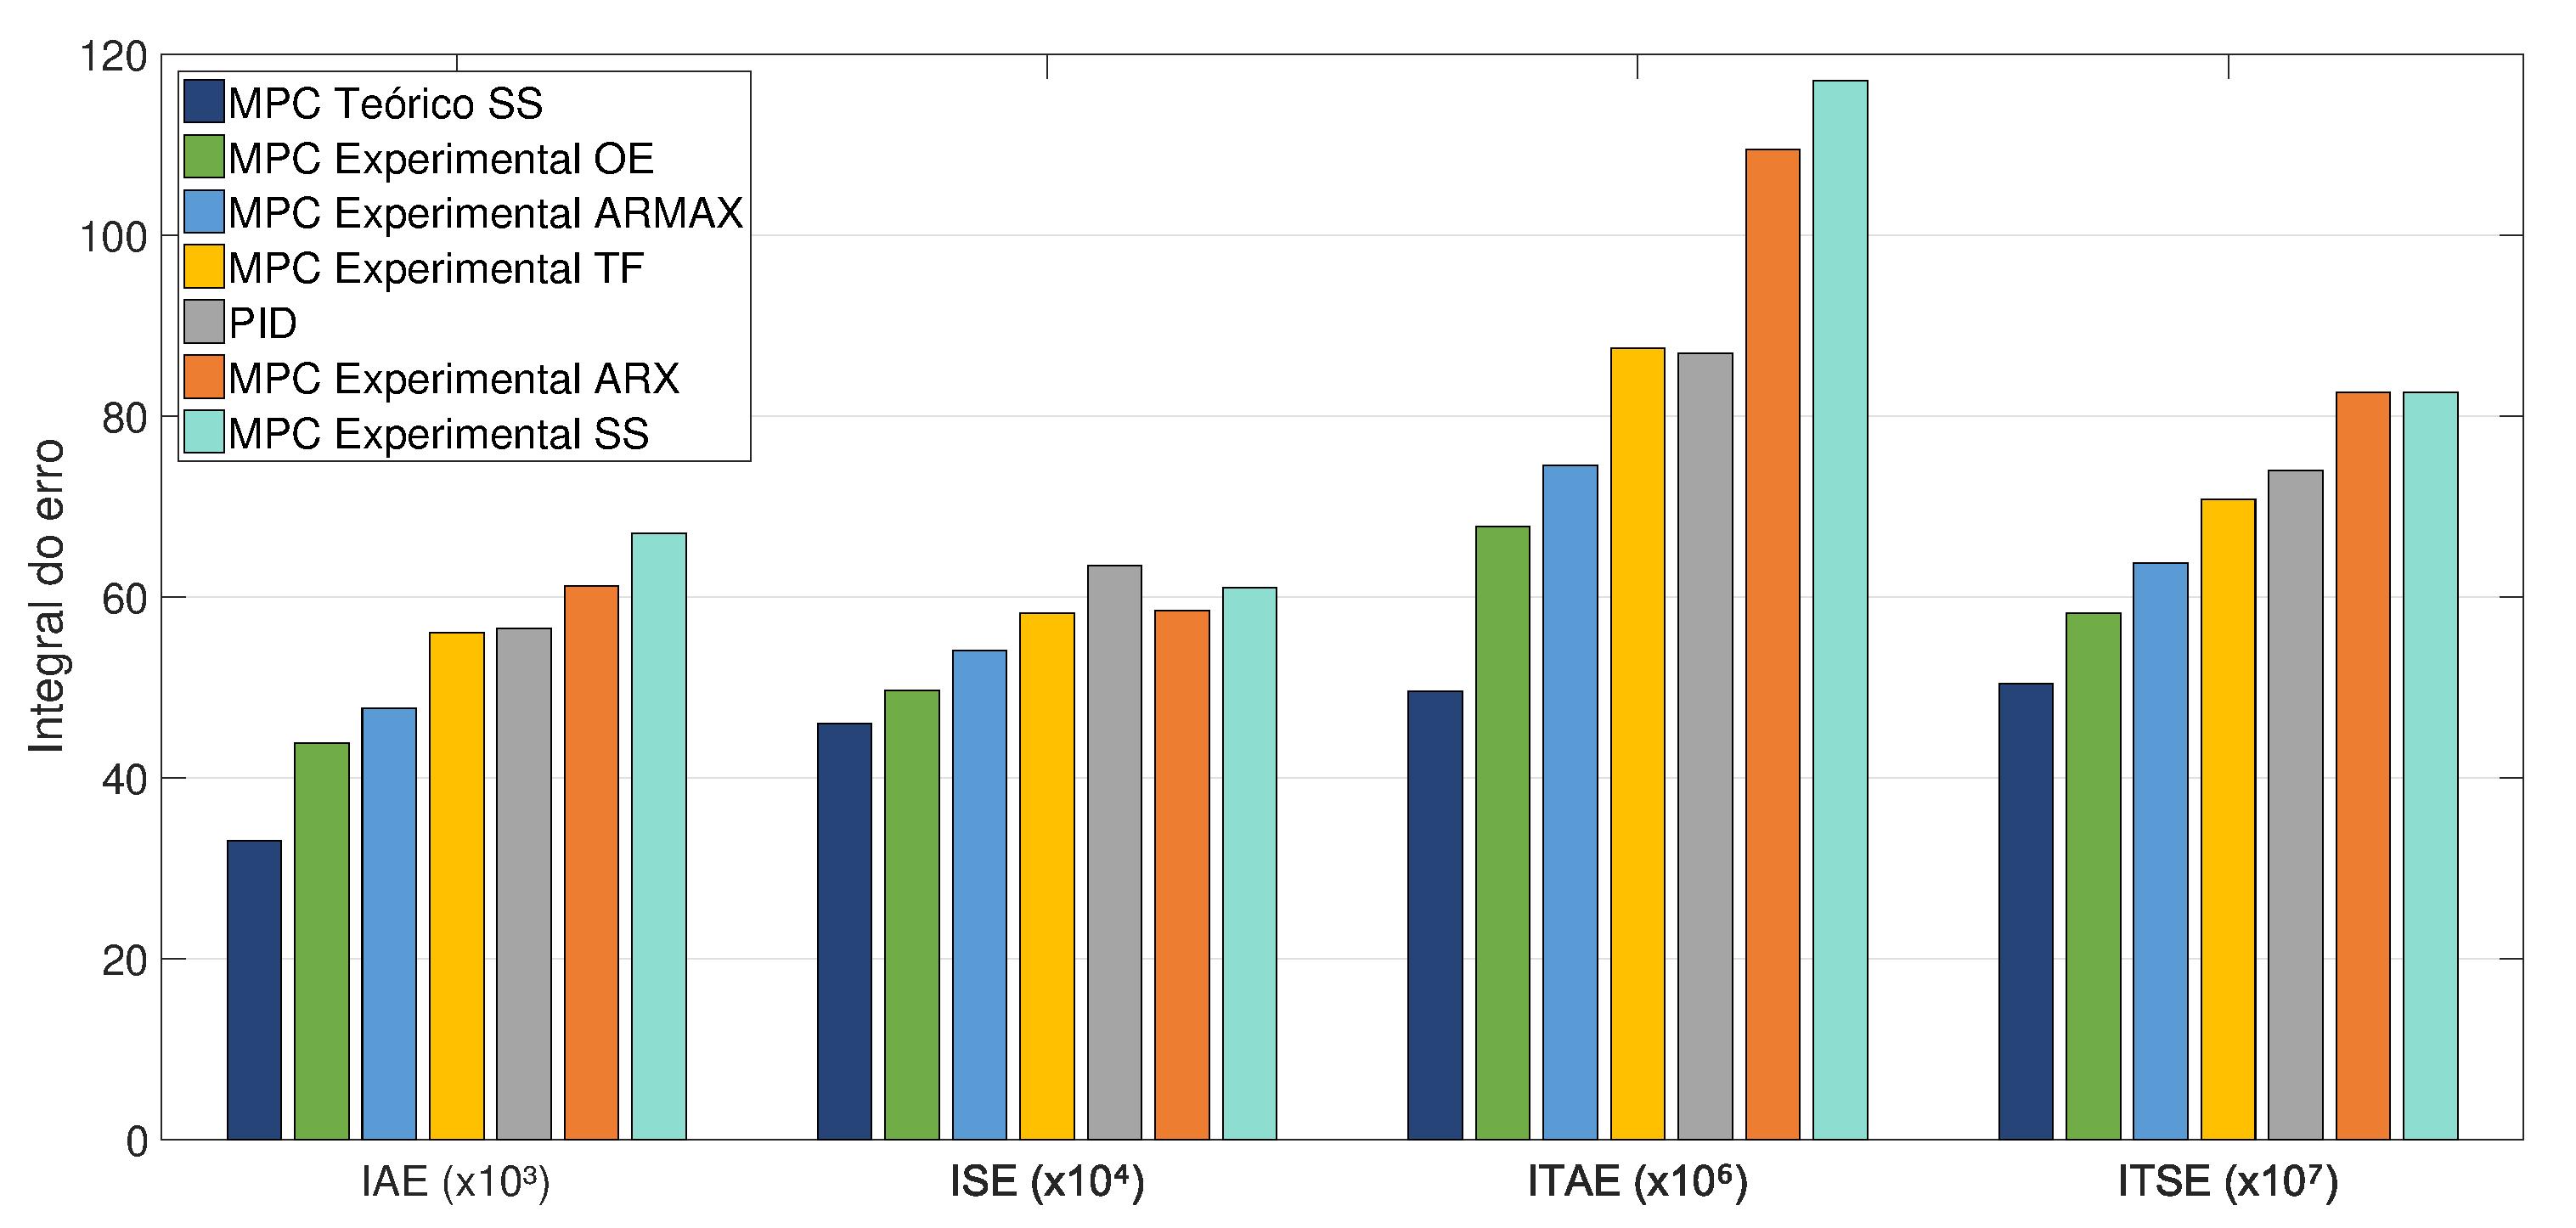
\includegraphics[width=1.00\textwidth]{./5_images/ResultadosPerformance.eps} 
		\label{fig:resultados_performance}
	\end{center}
	\centering
	\makebox[\width]{Fonte: Autor} 
\end{figure}

\clearpage

A partir da \cref{fig:resultados_performance} é possível observar que dentre todos os controladores analisados,
o controlador \acrshort{mpc} criado a partir do modelo em espaço de estados e obtido por abordagem teórica
foi o aquele que mostrou melhor controle da planta estudada (menor erro relativo). Mesmo quando comparado com o controlador 
\acrshort{pid} de referência, o controle \acrshort{mpc} em questão mostrou uma maior velocidade para a estabilização
dos seus múltiplos sinais de saída. Contudo, vale ressaltar que este controlador \acrshort{pid} 
foi apenas sintonizado utilizando a função de \textit{auto-tunning} disponível no \acrshort{matlab}.
Um controlador \acrshort{pid} melhor parametrizado poderia ter uma performance muito mais próxima das 
performances obtidas nos controladores \acrshort{mpc}, pois segundo \citeonline{Shaaban2013} e
\citeonline{Taysom2017} a diferença na performance destes dois controles é muito pequena quando
a planta possui pouco ou nenhum atraso (como a planta utilizada neste estudo), porém quando os atrasos
na planta aumentam, a resposta do controlador \acrshort{pid} se degrada rapidamente.

Ainda comparando os controladores \acrshort{mpc} e \acrshort{pid}, além das performances de ambos poderem ser
diferenciadas devido ao atraso do sistema, \citeonline{Taysom2017} também apontam em seu estudo que os
controladores \acrshort{mpc} geralmente apresentam uma melhor resposta para sistemas \acrshort{mimo},
além de serem mais efetivos em sistemas onde os distúrbios podem ser modelados, uma vez que o
\acrshort{mpc} consegue utilizar o modelo do processo e o modelo do distúrbio conjuntamente para um 
controle mais assertivo. Em contrapartida os controladores \acrshort{pid} são relativamente mais
fáceis de sintonizar e muito mais fáceis de se implementar, além de possuírem resposta similar ao \acrshort{mpc}
em uma grande variedade de aplicações \cite{Taysom2017}.

Outro ponto de destaque para os controladores \acrshort{mpc} é a possibilidade da configuração de
restrições de atuação, algo que é impossível de se fazer utilizando um controle \acrshort{pid}.
No caso do uso de restrições, o controlador \acrshort{mpc} impede que a(s) saída(s) da planta controlada
ultrapassem limites indesejados, fazendo com que o \acrshort{mpc} seja uma opção de controle muito
interessante quando se deseja maximizar ou minimizar valores de produção sem que algumas variáveis
do processo atinjam ou ultrapassem limites indesejados.

Observa-se através das \crefrange{fig:resultadosmpc-exptf}{fig:resultadosmpc-exparx} que mesmo utilizando
uma metodologia consolidada academicamente para a criação do controle \acrshort{mpc} através de modelos
experimentais, a resposta em malha fechada pode não ser satisfatória. Nestas figuras é possível 
observar uma oscilação indesejada nas saídas da planta, além de erro estacionário em alguns casos.
Todavia, ferramentas como o \textit{MPC design} do \acrshort{matlab} podem auxiliar no desenvolvimento
de um controle \acrshort{mpc} através de um modelo experimental que ao ser empiricamente sintonizado
pode apresentar uma resposta satisfatória em malha fechada. A \cref{fig:resultadosmpcmanual-exptf}
apresenta o gráfico em malha fechada de um controlador \acrshort{mpc} utilizando o mesmo modelo experimental em
função de transferência apresentado no capítulo anterior, porém desta vez sintonizado empiricamente utilizando
a ferramenta \textit{MPC Design}. A \cref{fig:resultados_performance_com_manual} traz novamente a
comparação de performance dos controladores porém desta vez incluindo este novo modelo e revela que, apesar de uma
sintonia empírica, este controlador apresenta uma aproximação do \textit{set-point} bem superior em comparação
aos controladores baseados em  modelos experimentais que já havíam sido apresentados neste trabalho.
Observando ainda a \cref{fig:resultadosmpcmanual-exptf} é possível verificar uma menor oscilação da
variável manipulada (MV) em comparação com os demais controladores.

Algumas imagens do \textit{MPC Design}, as tabelas de performance de cada um dos indicadores
incluindo este modelo empírico e o método de sintonia podem ser encontrados no \cref{ch:mpc_experimental_empirico}.

\begin{figure}[!h]
	\caption{Resposta do controlador MPC criado empiricamente a partir do modelo experimental (função de transferência)}
	\begin{center}
		\includegraphics[width=1.00\textwidth]{./5_images/ResultadosMPCManual-ExpTF.eps} 
		\label{fig:resultadosmpcmanual-exptf}
	\end{center}
	\centering
	\makebox[\width]{Fonte: Autor} 
\end{figure}

\begin{figure}[!h]
	\caption{Performance dos controladores MPC e PID agrupados por índice - Incluindo modelo empírico}
	\begin{center}
		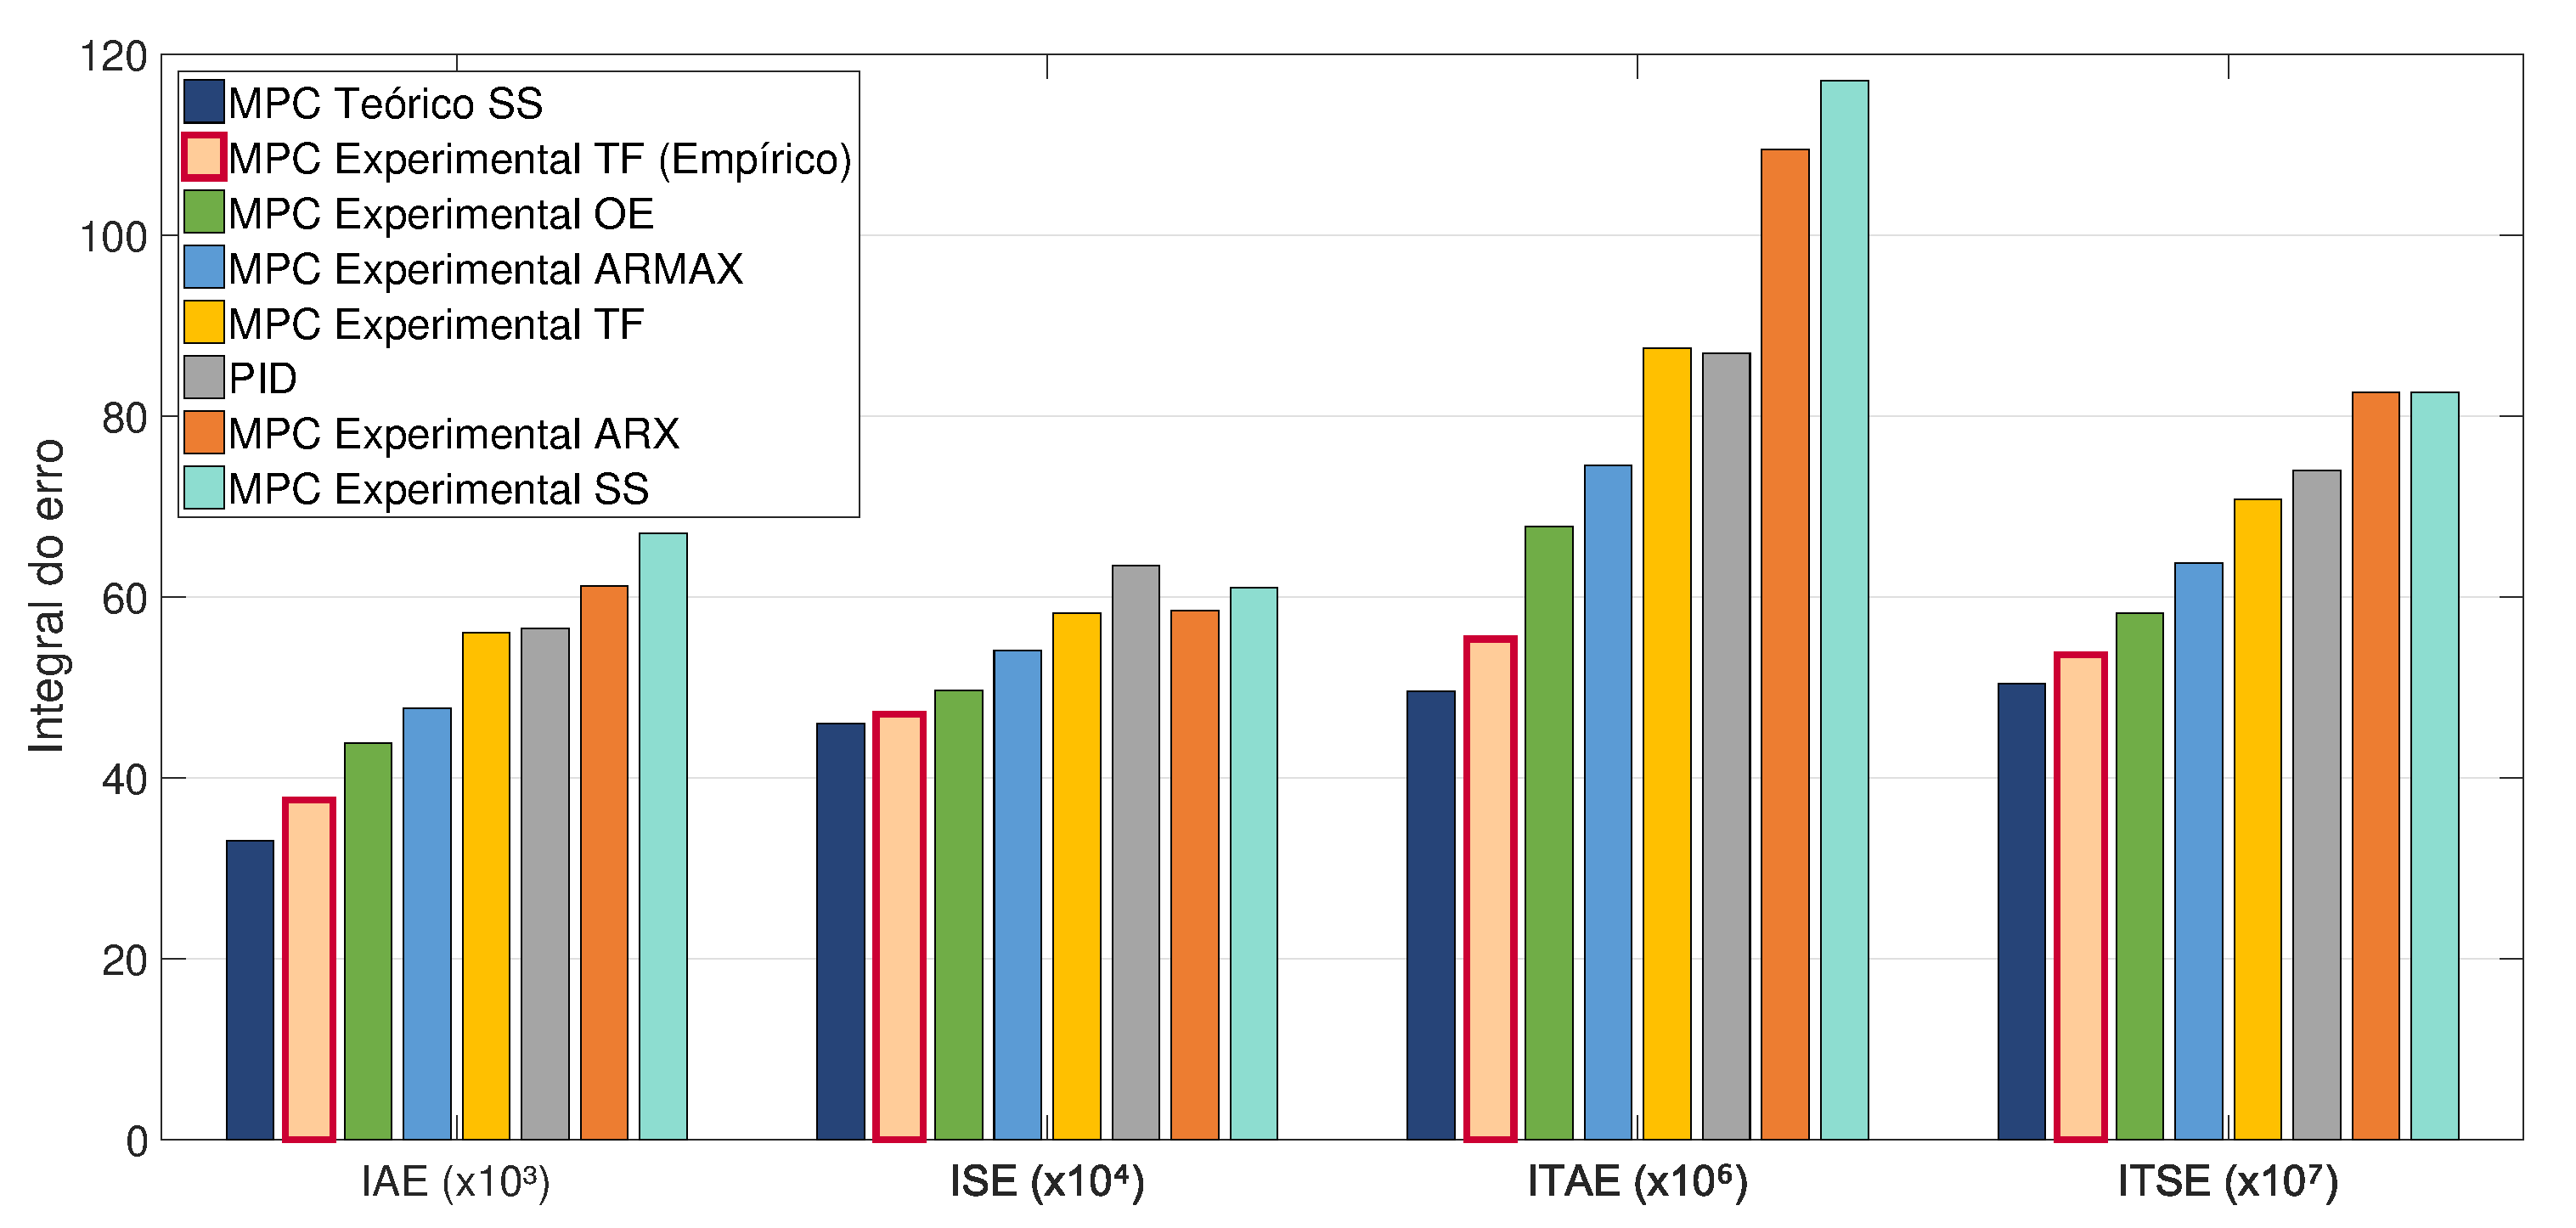
\includegraphics[width=1.00\textwidth]{./5_images/ResultadosPerformance_comManual.eps} 
		\label{fig:resultados_performance_com_manual}
	\end{center}
	\centering
	\makebox[\width]{Fonte: Autor} 
\end{figure}

Nota-se também neste controlador\footnote{
    Parâmetros encontrados empiricamente e ajustados para este controlador: Tempo de amostragem ($t_s$) = 2s; Horizonte de predição = 120;
    Horizonte de Controle = 16; $\Delta$ = 0; R = 0,4393; Q = 0,2276.
} apresentado na \cref{fig:resultadosmpcmanual-exptf} uma maior estabilidade
das variáveis manipuladas, apesar de um \textit{overshoot} maior que os demais controles.

De forma geral é possível afirmar que os objetivos deste trabalho foram alcançados com êxito, uma vez que foi
possível desenvolver e implementar um controle \acrshort{mpc} na planta desejada, comparar este controle 
com um controle \acrshort{pid} convencional e ainda documentar todas as etapas de forma que essas possam ser reproduzidas
por outros estudantes que estejam pesquisando sobre o \acrlong{mpc}.

% Comentários do Brincalepe
% Falar de possíveis melhorias futuras. (Sintonizar melhor o PID, Alterar a planta para ter atraso, modelar ruido, etc)			[ok]
% Detalhar MPC Design. Como foi feita a simulação empírica																		[ok]
% Avaliar se vale a pena alterar a função FIT por IAE (integral absolute error) 												[ok]
% Fazer versão digital de lado único para a defesa.																				[ok]

% =====================================================================================================
% ============================================= Chapter ===============================================
% =====================================================================================================
\chapter{Discussões}
\label{ch:discussoes}

Como recomendação para trabalhos futuros, deixo as seguintes sugestões abaixo:

\begin{itemize}
	\item \textbf{Realizar a sintonia fina do \acrshort{pid}}. O controlador \acrshort{pid} apresentou um
			desempenho bem inferior a maioria dos controladores \acrshort{mpc} desenvolvidos. Essa diferença
			pode diminuir significativamente caso o controlador \acrshort{pid} esteja bem sintonizado, tornando
			assim a comparação entre ambos os métodos mais próxima.
	\item \textbf{Modelar distúrbios}. O \acrshort{tclabsp} está equipado com ventiladores que podem
			atuar como distúrbios observáveis na planta. Modelar estes distúrbios e fazer com que o \acrshort{mpc}
			atue sobre eles pode aumentar bastante a robustez do projeto, além agregar muito conhecimento de
			situações industriais reais para quem o desenvolver.
	\item \textbf{Modificar a planta para aumentar o atraso}. Como visto no capítulo de resultados, o desempenho do
			controle \acrshort{mpc} pode ser mais expressivo, em comparação com o \acrshort{pid}, principalmente em
			plantas com atraso. Sendo assim, seria possível fazer algumas modificações no \acrshort{tclab} para que
			os sensores captem a mudança de temperatura dos aquecedores mais tardiamente. Uma das formas de se fazer
			isso seria inserindo entre os aquecedores e sensores algum material de condução térmica reduzida.
	\item \textbf{Testar diferentes sintonias para os controladores \acrshort{mpc}}. Ao concluir este trabalho
			observou-se que os modelos \acrshort{mpc} experimentais sintonizados com base na bibliografia
			tiveram uma performance inferior ao modelo sintonizado empiricamente. Atualmente existem diversos estudos
			que apresentam diferentes técnicas e metodologias para a sintonia de um controlador \acrshort{mpc}.
			Aplicar técnicas diferentes das usadas neste trabalho podem resultar em uma melhora na performance
			do controlador para os modelos experimentais.
\end{itemize}